\documentclass[10pt,openany]{book}\usepackage[]{graphicx}\usepackage[]{color}
% maxwidth is the original width if it is less than linewidth
% otherwise use linewidth (to make sure the graphics do not exceed the margin)
\makeatletter
\def\maxwidth{ %
  \ifdim\Gin@nat@width>\linewidth
    \linewidth
  \else
    \Gin@nat@width
  \fi
}
\makeatother

\definecolor{fgcolor}{rgb}{0.345, 0.345, 0.345}
\newcommand{\hlnum}[1]{\textcolor[rgb]{0.686,0.059,0.569}{#1}}%
\newcommand{\hlstr}[1]{\textcolor[rgb]{0.192,0.494,0.8}{#1}}%
\newcommand{\hlcom}[1]{\textcolor[rgb]{0.678,0.584,0.686}{\textit{#1}}}%
\newcommand{\hlopt}[1]{\textcolor[rgb]{0,0,0}{#1}}%
\newcommand{\hlstd}[1]{\textcolor[rgb]{0.345,0.345,0.345}{#1}}%
\newcommand{\hlkwa}[1]{\textcolor[rgb]{0.161,0.373,0.58}{\textbf{#1}}}%
\newcommand{\hlkwb}[1]{\textcolor[rgb]{0.69,0.353,0.396}{#1}}%
\newcommand{\hlkwc}[1]{\textcolor[rgb]{0.333,0.667,0.333}{#1}}%
\newcommand{\hlkwd}[1]{\textcolor[rgb]{0.737,0.353,0.396}{\textbf{#1}}}%
\let\hlipl\hlkwb

\usepackage{framed}
\makeatletter
\newenvironment{kframe}{%
 \def\at@end@of@kframe{}%
 \ifinner\ifhmode%
  \def\at@end@of@kframe{\end{minipage}}%
  \begin{minipage}{\columnwidth}%
 \fi\fi%
 \def\FrameCommand##1{\hskip\@totalleftmargin \hskip-\fboxsep
 \colorbox{shadecolor}{##1}\hskip-\fboxsep
     % There is no \\@totalrightmargin, so:
     \hskip-\linewidth \hskip-\@totalleftmargin \hskip\columnwidth}%
 \MakeFramed {\advance\hsize-\width
   \@totalleftmargin\z@ \linewidth\hsize
   \@setminipage}}%
 {\par\unskip\endMakeFramed%
 \at@end@of@kframe}
\makeatother

\definecolor{shadecolor}{rgb}{.97, .97, .97}
\definecolor{messagecolor}{rgb}{0, 0, 0}
\definecolor{warningcolor}{rgb}{1, 0, 1}
\definecolor{errorcolor}{rgb}{1, 0, 0}
\newenvironment{knitrout}{}{} % an empty environment to be redefined in TeX

\usepackage{alltt}

%\input{c:/aaaWork/zGnrlLatex/BookPreamble_HC}   % use for the hard-copy version
\input{c:/aaaWork/zGnrlLatex/BookPreamble}
\hypersetup{pdftitle = MTH107 Notes,bookmarksdepth=0}
\input{c:/aaaWork/zGnrlLatex/JustRPreamble}
\usepackage{animate}
\usepackage{titlesec}
\titlespacing\section{0pt}{12pt plus 4pt minus 2pt}{0pt plus 2pt minus 2pt}
\titlespacing\subsection{-3pt}{12pt plus 4pt minus 2pt}{0pt plus 2pt minus 2pt}
\titlespacing\subsubsection{-3pt}{12pt plus 4pt minus 2pt}{0pt plus 2pt minus 2pt}
\renewcommand{\chaptername}{Module}
\IfFileExists{upquote.sty}{\usepackage{upquote}}{}
\begin{document}




  \frontmatter
    %MAKE MINI TABLE OF CONTENTS for each chapter ----------------------------------
\dominitoc
\setcounter{minitocdepth}{1} %sets the depth to show in chapter TOC -- 0 is chapters, 1 would be sections, etc.

\VerbatimFootnotes  % allows verbatim in footnotes

%TITLE PAGE --------------------------------------------------------------------
\begin{titlepage}
\begin{center}

% Upper part of the page
\textsc{\LARGE Northland College}\\[0.5cm]
\textsc{\Large MTH107 -- Statistical Analysis and Interpretation}\\[1.5cm]

\HRuleW \\
\HRule \\[1cm]
{ \huge \bfseries Introduction to Statistical Analysis and Interpretation}\\[1cm]
\HRule \\
\HRuleW \\[1.5cm]

% Author and supervisor
\begin{minipage}{0.4\textwidth}
\begin{flushleft}
%  \Large \emph{Author:}\\ Dr. Derek H. Ogle
  \Large \emph{Instructors:}\\Dr. Derek H. Ogle \\ Jodi Supanich
\end{flushleft}
\end{minipage}
\begin{minipage}{0.4\textwidth}
\begin{flushright}
  \Large \emph{Department:} \\ Mathematical Sciences
%  \Large \emph{Department:} \\ Mathematical Sciences \\ Mathematical Sciences
\end{flushright}
\end{minipage}

\vfill

% Bottom of the page
%\includegraphics[width=4in]{Title.JPG} \\[2.5cm]
{\Large \today}

\end{center}

\end{titlepage}

% The material in the Preface_OLD.tex file was between here
% and here

%TABLE OF CONTENTS ---------------------------------------------------------------------------------------------------
\setcounter{tocdepth}{0} %sets the depth to show in TOC -- 0 is chapters, 1 would be sections, etc.

%modify what the parts look like
\renewcommand{\cftpartfont}{\scshape}                          %changes to small caps

%modify what the chapters look like
\setlength{\cftchapindent}{1.5em}                              %indent the chapters
\setlength{\cftbeforechapskip}{0.4em}                          %set the space between chapters -- reduce to 0.2 if depth is set to 0

%modify what the sections look like
\setlength{\cftsecindent}{3.8em}                               %indent the sections --- doesn't seem to work
\setlength{\cftbeforesecskip}{0.2em}                           %set the space between sections

\newpage                                                       %need this so that the TOC will start on its own page
\tableofcontents                                               %build the table of contents

%SETTING FOR LEAVING FRONT MATTER AND GOING TO MAIN DOCUMENT ---------------------------------------------------------
\addtocontents{toc}{\setlength{\cftbeforepartskip}{1.5em}}     %increase distance before parts in the main TOC
\addtocontents{toc}{\cftpagenumbersoff{part}}                  %so page numbers won't appear for parts in the main TOC


  \mainmatter


















\chapter{1-Sample t-Test} \label{chap:tTest1}

\minitoc
\vspace*{48pt}

\lettrine{P}{rior to this module}, hypothesis testing methods required knowing $\sigma$, which is a parameter that is seldom known. When $\sigma$ is replaced by its estimator, $s$, the test statistic follows a Student's t rather than a standard normal (Z) distribution. In this module, the t-distribution is described and a 1-Sample t-Test for testing that the mean from one population equals a specific value is discussed.

\vspace*{12pt}
\section{t-distribution}\label{sect:tDist}
A t-distribution is similar to a standard normal distribution (i.e., N(0,1)) in that it is centered on 0 and is bell shaped \figrefp{fig:tvsZ}. The t-distribution differs from the standard normal distribution in that it is heavier in the tails, flatter near the center, and its exact dispersion is dictated by a quantity called the degrees-of-freedom (df). The t-distribution is ``flatter and fatter'' because of the uncertainty surrounding the use of $s$ rather than $\sigma$ in the standard error calculation.\footnote{Recall that the sample standard deviation is a statistic and is thus subject to sampling variability.} The degrees-of-freedom are related to $n$ and generally come from the denominator in the standard deviation calculation. As the degrees-of-freedom increase, the t-distribution becomes narrower, taller, and approaches the standard normal distribution \figrefp{fig:tvsZ}.

\begin{knitrout}
\definecolor{shadecolor}{rgb}{0.922, 0.922, 0.922}\color{fgcolor}\begin{figure}[hbtp]

{\centering 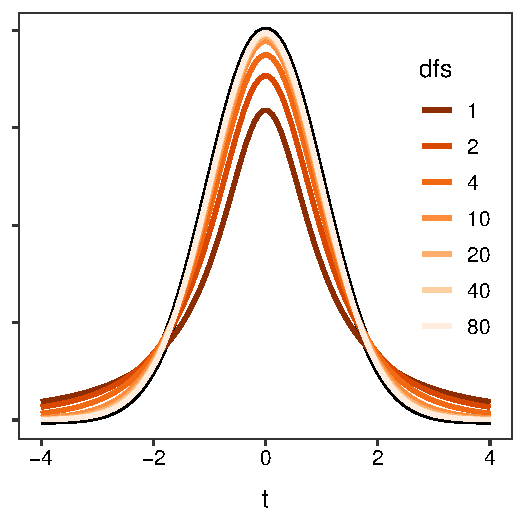
\includegraphics[width=.4\linewidth]{Figs/tvsZ-1} 

}

\caption[Standard normal (black) and t-distributions with varying degrees-of-freedom]{Standard normal (black) and t-distributions with varying degrees-of-freedom.}\label{fig:tvsZ}
\end{figure}


\end{knitrout}

\newpage
\vspace*{12pt}
Proportional areas on a t-distribution are computed using \R{distrib()} similar to what was described for a normal distribution in Modules \ref{chap:NormDist} and \ref{chap:SamplingDist}. The major exceptions for using \R{distrib()} with a t-distribution is that \R{distrib="t"} must be used and the degrees-of-freedom must be given in \R{df=} (how to find df is discussed in subsequent sections). For example, the area right of $t=-1.456$ on a t-distribution with 9 df is 0.9103 \figrefp{fig:tarea1}.
\begin{knitrout}
\definecolor{shadecolor}{rgb}{0.922, 0.922, 0.922}\color{fgcolor}\begin{kframe}
\begin{verbatim}
> ( distrib(-1.456,distrib="t",df=9,lower.tail=FALSE) )
[1] 0.9103137
\end{verbatim}
\end{kframe}\begin{figure}[hbtp]

{\centering 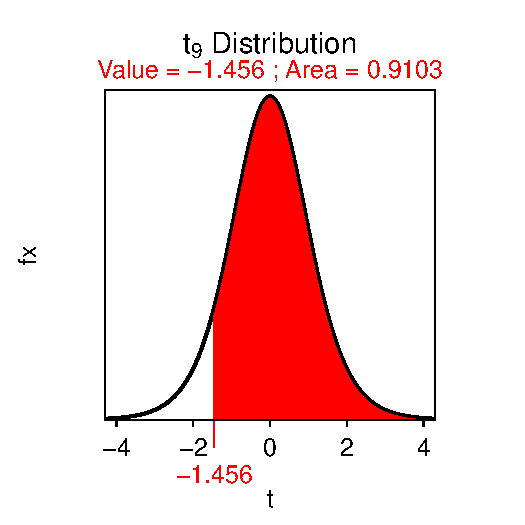
\includegraphics[width=.4\linewidth]{Figs/tarea1-1} 

}

\caption[Depiction of the area to the right of $t=-1.456$ on a t-distribution with 9 df]{Depiction of the area to the right of $t=-1.456$ on a t-distribution with 9 df.}\label{fig:tarea1}
\end{figure}


\end{knitrout}

Similarly, the $t$ with an upper-tail area of 0.95 on a t-distribution with 19 df is -1.729 \figrefp{fig:tstar1}.\footnote{This ``reverse'' calculation would be $t^{*}$ for a 95\% lower confidence bound.}
\begin{knitrout}
\definecolor{shadecolor}{rgb}{0.922, 0.922, 0.922}\color{fgcolor}\begin{kframe}
\begin{verbatim}
> ( distrib(0.95,distrib="t",type="q",df=19,lower.tail=FALSE) )
[1] -1.729133
\end{verbatim}
\end{kframe}\begin{figure}[hbtp]

{\centering 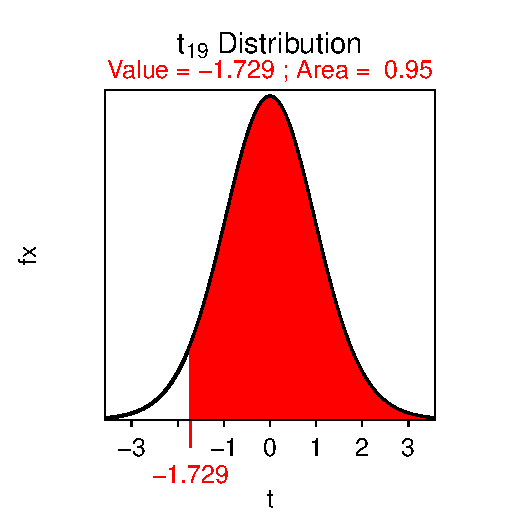
\includegraphics[width=.4\linewidth]{Figs/tstar1-1} 

}

\caption[Depiction of the value of t with an area to the right of 0.95 on a t-distribution with 19 df]{Depiction of the value of t with an area to the right of 0.95 on a t-distribution with 19 df.}\label{fig:tstar1}
\end{figure}


\end{knitrout}


\section{1-Sample t-Test Specifics} \label{sect:t1test}
A 1-Sample t-Test is similar to a 1-Sample Z-test in that both test the same $H_{0}$. The difference, as discussed above, is that when $\sigma$ is replaced by $s$, the test statistic becomes $t$ and the scaling factor for confidence regions becomes a $t^{*}$. Other aspects are similar between the two tests as shown in \tabref{tab:1tspec}.\footnote{Compare \tabref{tab:1tspec} to \tabref{tab:1Zspec}.}

\begin{table}[h]
\centering
\colorbox{ltgray}{
\begin{minipage}{.75\textwidth}
  \centering
	\caption{Characteristics of a 1-Sample t-Test.}\label{tab:1tspec}
  \begin{Itemize}
    \vspace*{-6pt}
      \item \textbf{Hypothesis:} $H_{0}:\mu=\mu_{0}$
      \item \textbf{Statistic:} $\bar{x}$
      \vspace{4pt}
      \item \textbf{Test Statistic:} $t=\frac{\bar{x}-\mu_{0}}{\frac{s}{\sqrt{n}}}$
      \vspace{4pt}
      \item \textbf{Confidence Region:} $\bar{x}+t^{*}\frac{s}{\sqrt{n}}$
      \item \textbf{df}: $n-1$
      \item \textbf{Assumptions:}
        \begin{Enumerate}
          \item $\sigma$ is UNknown
          \item $n\geq40$, $n\geq15$ and the \textbf{sample} (i.e., histogram) is not strongly skewed, OR the \textbf{sample} is normally distributed.
        \end{Enumerate}
      \item \textbf{Use with:} Quantitative response, one group (or population), $\sigma$ UNknown.
  \end{Itemize}
\end{minipage}}
\end{table}

\section{Examples}
\vspace{-8pt}
\subsection{Purchase Catch of Salmon?}
Below are the 11-steps \sectrefp{sec:11Steps} for completing a full hypothesis test for the following situation:
\begin{quote}
\textsl{A prospective buyer will buy a catch of several thousand salmon if the mean weight of all salmon in the catch is at least 19.9 lbs. A random selection of 50 salmon had a mean of 20.1 and a standard deviation of 0.76 lbs. Should the buyer accept the catch at the 5\% level?}
\end{quote}
\vspace*{-12pt}

\begin{Enumerate}
    \item $\alpha$=0.05.
    \item $H_{0}:\mu=19.9$ lbs vs. $H_{A}:\mu >19.9$ lbs where $\mu$ is the mean weight of ALL salmon in the catch.
    \item A 1-Sample t-Test is required because (1) a quantitative variable (weight) was measured, (ii) individuals from one group (or population) were considered (this catch of salmon), and (iii) $\sigma$ is \textbf{UN}known.\footnote{If $\sigma$ is given, then it will appear in the background information to the question and will be in a sentence that uses the words ``population'', ``assume that'', or ``suppose that.''}
    \item The data appear to be part of an observational study with random selection.
    \item (i) n=50 $\geq$ 40 and (ii) $\sigma$ is unknown.
    \item $\bar{x}$ = 20.1 lbs (and $s$ = 0.76 lbs).
    \item $t$ = $\frac{20.1-19.9}{\frac{0.76}{\sqrt{50}}}$ = $\frac{0.2}{0.107}$ = 1.87 with df = 50-1 = 49.
    \item p-value = $0.0337$. [\textit{See R code in appendix.}]
    \item $H_{0}$ is rejected because the p-value $< \alpha$.
    \item The average weight of ALL salmon in this catch appears to be greater than 19.9 lbs; thus, the buyer should accept this catch of salmon.
    \item I am 95\% confident that the mean weight of ALL salmon in the catch is greater than 19.92 lbs (i.e., $20.1-1.677\frac{0.76}{\sqrt{50}}$ = $20.1-0.18$ = $19.92$). [\textit{See R code in appendix.}]
\end{Enumerate}

\vspace{-6pt}
\begin{minipage}{\textwidth}
\textbf{R Appendix:}
\vspace{-6pt}
\begin{knitrout}
\definecolor{shadecolor}{rgb}{0.922, 0.922, 0.922}\color{fgcolor}\begin{kframe}
\begin{verbatim}
( pval <- distrib(1.87,distrib="t",df=49,lower.tail=FALSE) )
( tstar <- distrib(0.95,distrib="t",type="q",df=49,lower.tail=FALSE) )
\end{verbatim}
\end{kframe}
\end{knitrout}
\end{minipage}


\subsection{Body Temperature}
\vspace*{-4pt}
Below are the 11-steps \sectrefp{sec:11Steps} for completing a full hypothesis test for the following situation:
\vspace*{-8pt}
\begin{quote}
\textsl{Machowiak et al. (1992) critically examined the belief that the mean body temperature is 98.6$^{o}$F by measuring body temperatures in a sample of healthy humans. Use their results in \tabref{tab:1ttemp} to determine at the 1\% level if the mean body temperature differs from 98.6$^{o}$F.}
\end{quote}

\vspace*{-4pt}
\begin{table}[h]
  \caption{Results from measuring the body temperature of a sample of healthy humans.}
  \label{tab:1ttemp}
  \vspace*{-12pt}
\begin{knitrout}
\definecolor{shadecolor}{rgb}{1, 1, 1}\color{fgcolor}\begin{kframe}
\begin{verbatim}
     n   mean     sd    min     Q1 median     Q3    max 
130.00  98.25   0.73  96.30  97.80  98.30  98.70 100.80 
\end{verbatim}
\end{kframe}
\end{knitrout}
\end{table}


\begin{Enumerate}
  \item $\alpha$=0.01.
  \item $H_{0}:\mu=98.6^{o}$F vs. $H_{A}:\mu\neq98.6^{o}$F, where $\mu$ is the mean body temperature for ALL healthy humans. [\textit{Note that not equals was used because the researchers want to determine if the temperature is \textbf{different from} $98.6^{o}$F.}]
  \item A 1-Sample t-Test is required because (i) a quantitative variable (i.e., body temperature) was measured, (ii) individuals from one group (or population) is considered (i.e., healthy humans), and (iii) $\sigma$ is unknown (i.e., not given in the background).
  \item The data appear to be part of an observational study although this is not made clear in the background information. There is also no evidence that randomization was used.
  \item (i) $n=130\geq40$ and (ii) $\sigma$ is unknown.
  \item $\bar{x}$ = 98.25$^{o}$F.
  \item $t$ = $\frac{98.25-98.6}{\frac{0.73}{\sqrt{130}}}$ = $\frac{-0.35}{0.064}$ = -5.469 with df = 130-1 = 129.
  \item p-value=$0.0000002$. [\textit{See R code in appendix. Note that the result of \r{distrib()} is multiplied by 2 because of the not equals $H_{A}$.}]
  \item Reject $H_{0}$ because p-value$<\alpha=0.01$.
  \item It appears that the mean body temperature of ALL healthy humans is less than 98.6$^{o}$F. [\textit{Note that the test was for a difference but because $\bar{x}<98.6$ this more specific conclusion can be made.}]
  \item I am 99\% confident that the mean body temperature ($\mu$) for ALL healthy humans is between 98.08$^{o}$C (=98.25-2.614*0.064) and 98.42$^{o}$C (=98.25+2.614*0.064). [\textit{See R code in appendix. Note that the area in \r{distrib()} is $1-\frac{\alpha}{2}$ because of the not equals $H_{A}$.}]
\end{Enumerate}

\begin{minipage}{\textwidth}
\textbf{R Appendix:}
\vspace*{-6pt}
\begin{knitrout}
\definecolor{shadecolor}{rgb}{0.922, 0.922, 0.922}\color{fgcolor}\begin{kframe}
\begin{verbatim}
( pval <- 2*distrib(-5.469,distrib="t",df=130) )
(tstar <- distrib(0.995,distrib="t",df=130) )
\end{verbatim}
\end{kframe}
\end{knitrout}
\end{minipage}





%    \cleardoublepage
%    \phantomsection
%    \addcontentsline{toc}{part}{Appendix}
%    \chapter*{Appendices}
%    \appendix


%  \backmatter
%    %BIBLIOGRAPHY ---------------------------------------------------------------------------------------------------------
\cleardoublepage                             %not sure why but this is needed so TOC entry will point to right start page
\phantomsection                              %not sure why but this is needed so TOC entry will point to right start page
\addcontentsline{toc}{part}{Bibliography}    %Add a TOC entry
\bibliography{c:/aaaWork/zGnrlLatex/DHO_Bib} %make the bibliography
 
%INDEX ----------------------------------------------------------------------------------------------------------------
% cross references for the index
\index{Alternative Hypothesis|see{Hypothesis, Alternative}}
\index{Coefficient of Determination|see{$r^{2}$}}
\index{Forward calculation|see{Normal Distribution, Finding areas}}
\index{Frequency Table|see{Table, Frequency}}
\index{Goodness-of-Fit Test|see{Chi-square}}
\index{Line!Finding best-fit|see{Regression}}
\index{Mean!Inference|see{Z-test and t-Test}}
\index{Null Hypothesis|see{Hypothesis, Null}}
\index{Percentage Table|see{Table}}
\index{Proportions Table|see{Table, Proportion}}
\index{Row Proportions Table|see{Table, Proportion}}
\index{Column Proportions Table|see{Table, Proportion}}
\index{Table Proportions Table|see{Table, Proportion}}
\index{Proportions, Inference|see{Chi-square}}
\index{Rejection Criterion|see{$\alpha$}}
\index{Reverse calculation|see{Normal Distribution, Finding values}}
\index{Simple Linear Regression|see{Regression}}
\index{SLR|see{Regression}}
\index{Standard Normal Distribution|see{Normal Distribution}}
\index{Standardization|see{Normal Distribution, Converting to Z-scale}}
\index{One-sample Z-Test|see{Z-Test}}
\index{1-sample Z-Test|see{Z-Test}}
\index{One-sample t-Test|see{t-Test}}
\index{1-sample t-Test|see{t-Test}}
\index{Two-sample t-Test|see{t-Test}}
\index{2-sample t-Test|see{t-Test}}
\index{Matched-Pairs t-Test|see{t-Test}}
\index{Two-way Table|see{Table, Frequency}}
\index{Type I Error|see{Hypothesis Testing, Errors}}
\index{Type II Error|see{Hypothesis Testing, Errors}}
\index{Variability!Natural|see{Natural Variability}}
\index{Variability!Sampling|see{Sampling Variability}}
\index{Variable!Types|see{Quantitative, Continuous, Discrete, Categorical, Nominal, or Ordinal}}
\index{Variance!Testing Equality|see{Levene's Test}}
\index{Y-intercept|see{Intercept}}
\index{Z-Distribution|see{Normal Distribution, Standard Normal}}

% code to actually add the index
\addtocontents{toc}{\setlength{\cftbeforepartskip}{0.4em}}  %decrease dist before parts in back matter portion of TOC
\cleardoublepage                          %not sure why but this is needed so TOC entry will point to right start page
\phantomsection                           %not sure why but this is needed so TOC entry will point to right start page
\addcontentsline{toc}{part}{Index}        %Add a TOC entry
\printindex                               %Make the index


\end{document}
